% !TEX encoding = UTF-8
% !TEX TS-program = pdflatex
% !TEX root = ../tesi.tex
% !TEX spellcheck = it-IT

%************************************************
\chapter{Classificazione}
\label{cap:ctbnc}
%************************************************
In questo capitolo viene introdotta una classe di modelli, che prende il nome di \acf{CTBNC}, il cui scopo è la classificazione supervisionata di traiettorie multivariate di variabili discrete a tempo continuo e spazio degli stati discreto. Si descrivono due istanze di tale classe: i classificatori \acf{CTNB} nella \autoref{sec:learning-ctnb} e i classificatori \acf{CTTANB} nella \autoref{sec:learning-cttanb}, per le quali si affronta il processo di apprendimento in caso di dati completi.

Infine, nella \autoref{sec:inference-ctbnc}, si presenta un algoritmo di inferenza esatta per la classe dei \acs{CTBNC}.

\section{Apprendimento}
Ciao!

\begin{figure}
\centering
\includegraphics[width=0.9\columnwidth]{immagini/ctbnc}
\caption[Un esempio di \acs{CTBNC}]{Un esempio di \acl{CTBNC} con cinque nodi attributo, $\setel{X}_1\,,\,\dotsc\,,\,\setel{X}_5$, e un nodo classe, $\setel{Y}$.}
\label{fig:ctbnc-example}
\end{figure}

\subsection{Na\"ive Bayes}\label{sec:learning-ctnb}
...

\begin{figure}
\centering
\includegraphics[width=0.9\columnwidth]{immagini/ctnb}
\caption[Un \acs{CTNB} \class{}]{Un \acl{CTNB} \class{}.}
\label{fig:ctnb}
\end{figure}

\subsection{Tree Augumented Na\"ive Bayes}\label{sec:learning-cttanb}
...

\begin{figure}
\centering
\includegraphics[width=0.9\columnwidth]{immagini/cttanb}
\caption[Un \acs{CTTANB} \class{}]{Un \acl{CTTANB} \class{}: qualora la variabile classe $\setel{Y}$ venga rimossa, le variabili rimanenti formano un albero.}
\label{fig:cttanb}
\end{figure}

\section{Inferenza}\label{sec:inference-ctbnc}
...

\subsection{Na\"ive Bayes}\label{sec:inference-ctnb}
...


% TODO
% They implement a trade-off between computational complexity and classification accuracy.
% The performance of the continuous time naive Bayes classifier is assessed in the case where real-time feedback to neurological patients undergoing motor rehabilitation must be provided
